\chapter{Data models and transformations}

The data about the academic researchers and their publications at CUNI is internally stored in a relational database. 
The first chapter of this thesis explores the transformation of the relational data model into a graph data model, 
which will allow us to use the graph algorithms for the social network analysis.

We also address pitfalls and challenges of the transformation stemming 
from the specific nature of the data and the technical limitations of the source systems.

\section{Input data format}

The Charles University information system is composed of a set of separate systems and applications.

The \textit{Studium} information system\footnote{Available at \url{https://is.cuni.cz/studium/}.} contains the data about the researchers, teachers, the courses and study programmes available at the university.

The \textit{Věda} information system\footnote{Available at \url{https://is.cuni.cz/veda/}, login only.} aggregates the data about creative activities of the researchers, the research projects and inter-university mobility programmes.
For the purpose of this thesis, we are mostly interested in the OBD (or Verso) module, containing the data about the academic publications.

The \textit{Whois} staff information system\footnote{Available at \url{https://is.cuni.cz/webapps/whois2}.} contains the data about the employees of the university, 
their affiliations with the faculties and departments and their academic titles.

While none of the systems offer public APIs, a data import pipeline has been set up by the university's IT department (ÚVT) in advance
for the purpose of the Charles Explorer application. 
This pipeline consists of a set of database views tracking the changes in the data and a script\footnote{\url{https://gitlab.mff.cuni.cz/barj/charles-explorer/-/blob/master/scripts/export.sh}} that exports the data to an SQLite database.

\newpage

\subsection{Exploring the schema}

To illustrate the structure of the data, we provide an example of the schema of the relational database together with example data.
Since this thesis focuses on the social network between the academic researchers and their publications, we limit this example only on the relevant parts of the schema.

The social network-relevant data accessible in the following three database views:

\begin{Verbatim}[commandchars=\\\{\}]
PERSON (
    \verbun{\verbbf{PERSON_ID}}, \verbxs{- UKČO personal number}
    PERSON_NAME, \verbxs{- Full name of the person, incl. the academic titles}
    PERSON_WEBSITE, \verbxs{- Personal website of the person}
    \verbun{\verbbf{PERSON_WHOIS_ID}}, \verbxs{- ID of the person in the Whois system}
    TYPE \verbxs{- Person type - teacher(U), external employee(E), or other(O)}
)
\end{Verbatim}

The \texttt{Person} view contains the data about the academic researchers and teachers at the university.
While the \texttt{TYPE} column might suggest that the table contains records about external people as well (e.g. guest co-authors of publications published by the CUNI researchers),
it only contains the data about the people affiliated with the university. The \texttt{TYPE} column is only used to distinguish between the different employment types at the university.

\begin{Verbatim}[commandchars=\\\{\}]
PUBLICATION_KEYWORDS (
    \verbun{\verbbf{PUBLICATION_ID}}, \verbxs{- internal ID of the publication}
    PUB_YEAR, \verbxs{- year of the publication}
    TITLE, \verbxs{- title of the publication}
    ABSTRACT, \verbxs{- abstract of the publication}
    KEYWORDS, \verbxs{- keywords of the publication}
    LANGUAGUE\verbxs{(sic!)}, \verbxs{- ISO 639-2 language code of the TITLE,}
                              \verbxs{ABSTRACT and KEYWORD columns}
    ORIGINAL\verbxs{ - whether the LANGUAGUE column is the original}
                               \verbxs{language of the publication}
)
\end{Verbatim}

This schema shows some more issues with the data - the \texttt{PUBLICATION\_KEYWORDS} is missing a single primary key attribute,
as the \texttt{PUBLICATION\_ID} is not unique across the table. This is because the same publication can have multiple records in the table,
each record representing a different language version of the title, abstract and keywords.

Moreover, the \texttt{PUBLICATION\_KEYWORDS} view does not contain an universally accepted publication identifier (e.g. a DOI or an ISBN) 
that would allow us to link the publication to the external sources of the publication data.
This is because of a technical limitation of the information systems, as the \textit{OBD} module is not fully interoperable with the \textit{Studium} module we are 
consuming the data from.

\newpage

\label{sec:pub-author-all}
\begin{Verbatim}[commandchars=\\\{\}]
PUBLICATION_AUTHOR_ALL (
    \verbun{PUBLICATION_ID}, \verbxs{- internal ID of the publication}
    \verbun{PERSON_ID}, \verbxs{- UKČO personal number of the author, if available}
    PERSON_NAME, \verbxs{- Full name of the author, incl. the academic titles}
)
\end{Verbatim}

The relational database view \texttt{PUBLICATION\_AUTHOR\_ALL} contains the links between the publications and the authors from the previous views.

With the most naive approach, the transformation of the relational data model into a graph data model could be done by transforming the records of the 
\texttt{PERSON} and (deduplicated) \texttt{PUBLICATION\_KEYWORDS} views into the nodes of the graph, 
and the records of the \texttt{PUBLICATION\_AUTHOR\_ALL} view into the edges of the graph.

\section{Transformation}

In the \hyperref[sec:pub-author-all]{comment} for the \texttt{PUBLICATION\_AUTHOR\_ALL.PERSON\_ID} column, we note that the UKČO personal number is not always available.
This is because of external authors, who are not affiliated with the university and do not have a UKČO personal number.
What is worse, such authors are only identified by their name and academic titles, which can be inconsistent across the publications.
This is again caused by the technical limitations of the source systems, as the interoperability between the \textit{OBD} and \textit{Studium} modules is limited.

This poses a challenge for the transformation of the relational data model into a graph data model, as we need to come up 
with a way to identify the external authors and link them to the publications.

\subsection{Inferring missing identities}

As mentioned above, the available relational data model is unfit for a direct transformation into a graph data model.
This is because the data about the external authors is incomplete and inconsistent, which might cause some of the authors
to be represented by multiple nodes in the graph.

Aside from the obvious implications of this issue - i.e. user confusion and potential performance issues,
this also poses a challenge for the social network analysis, as the graph algorithms might not be able 
to correctly identify the external authors.

In the aforementioned \texttt{PUBLICATION\_AUTHOR\_ALL} view, counts of the relations mentioning the authors with / without the UKČO personal number are as follows:

\begin{figure}[!ht]
    \captionsetup{width=.9\linewidth}
    \centering
    \begin{tabular}{|c|c|c|}
    \hline
        Type & Count & Distinct \\ \hline
        PERSON\_ID present & 808467 & 39523 \\ \hline
        PERSON\_ID missing & 671332 & ? \\ \hline
    \end{tabular}
    \caption{Counts of the relations in the \texttt{PUBLICATION\_AUTHOR\_ALL} view.}
\end{figure}

We see that the no-identifier authors take up to 45\% of the total count of the relations.
This explains the importance of the problem of inferring the missing identities.

\subsubsection{Naïve approach}

The naïve solution to this problem is using the \textit{names} for the identity inference 
in case of missing identifiers.
While this is a simple and straightforward transformation, it has obvious drawbacks.

Firstly, the names are not guaranteed to be \textit{unique} across the dataset. 

Secondly, the names are not guaranteed to be \textit{consistent} across the dataset - due to name changes (e.g. marital), 
typos, or different conventions in the academic titles.
See the example of a search for the name ``Jaroslav Peška'' in the \texttt{PUBLICATION\_AUTHOR\_ALL} view:

\begin{figure}[!ht]\label{fig:jaroslav-peska}
    \captionsetup{width=.9\linewidth}
    \centering
    \begin{tabular}{|c|c|c|}
    \hline
        COUNT(*) & PERSON\_NAME & PERSON\_ID \\ \hline
        2 & doc. PhDr. Jaroslav Peška Ph.D. & 14124313\dots \footnotemark \\ \hline
        5 & doc. PhDr. Jaroslav Peška Ph.D. & null \\ \hline
        2 & Doc. PhDr. Jaroslav Peška Ph.D. & null \\ \hline
        1 & doc. PhDr. Jaroslav Peška PhD. & null \\ \hline
        4 & Jaroslav Peška & null \\ \hline
    \end{tabular}
    \caption{Search for the name ``Jaroslav Peška'' in the \texttt{PUBLICATION\_AUTHOR\_ALL} view.}
\end{figure}

\footnotetext{PERSON\_ID redacted for privacy reasons, replaced by truncated PERSON\_WHOIS\_ID.}

While there are 5 variants of the same name in the dataset, only one of them is correctly linked to the UKČO personal number.
This could have been caused by human error on data input or by the limitations of the source systems. 
Either way, this creates an unrecoverable loss of information in the dataset.

In the SQL database export, we can ``merge'' the records using the naïve approach efficiently using a many-to-one (non-injective) mapping
on the \texttt{PERSON\_NAME} column.

Let us define a function $f$:
$$f: \text{PERSON\_NAME} \to \text{NORMALIZED\_NAME}$$

We require $f$ to map all person names to a \textit{normalized form}, which is defined as follows:
\begin{itemize}
    \item The academic titles are stripped from the name.
    \item The name is converted to lowercase.
    \item The name is stripped of any diacritics.
    \item The name is stripped of any non-alphabetic characters.
    \item The whitespace characters are normalized to a single space.
    \item The name is stripped of any leading or trailing whitespace.
\end{itemize}

We can see that in the case of \hyperref[fig:jaroslav-peska]{Jaroslav Peška}, 
the normalized version for all the variants is the same (i.e. $f(\texttt{PERSON\_NAME}) = \texttt{jaroslav peska}$).

If we decide to add the output of this normalization function as an attribute in the \texttt{PUBLICATION\_AUTHOR\_ALL} view,
we can proceed with the merging of the records using SQL GROUP BY and the aggregation functions.

% \label{infobox:sqlite-loadable-extensions}
\begin{mybox}
    {SQLite Loadable Extensions}

    While it would be possible to implement the normalization function using inbuilt scalar SQLite functions (namely \texttt{lower}, \texttt{trim},
    and repeated use of \texttt{replace}), the developer experience of such solution is suboptimal, as it requires a lot of nested function calls
    in the \texttt{SELECT} clause.

    Because the way the scalar functions are defined in SQLite - and their implementation\footnote{\url{https://sqlite.org/src/file?name=src/func.c}}, 
    the repeated calls to \texttt{replace} also result in repeated string allocations and deallocations - which can be a performance bottleneck.

    Fortunately, SQLite allows the user to define their own loadable extensions\footnote{\url{https://www.sqlite.org/loadext.html}} in C.
    This allows us to define the normalization function in C and load it as a scalar function in the SQLite database.
\end{mybox}

\textbf{Implementation}

For the implemetation of the name normalization function, we use the SQLite loadable extensions mechanism.
The string transformation itself is done in three steps:

\begin{enumerate}
    \item Using the \texttt{glib} function \texttt{g\_utf8\_normalize}, the string representation of the name is normalized to the canonical Unicode NFD form.
    This performs the Unicode decomposition of the diacritized letters and other characters. This step ensures that the byte representation of diacritized 
    characters is now composed of separate characters for the base character and the diacritics (e.g. \texttt{ě}\texttt{(U+011B)} is decomposed to \texttt{e}\texttt{(U+0065)} and \texttt{ˇ}\texttt{(U+02C7)}).
    \item We scan the normalized string and remove all the characters that are not in the range of the Latin alphabet. We convert the all the 
    alphabetic characters to lowercase and replace all the whitespace characters with a single space.
    \item Using regular expressions, we remove the academic titles from the name. 
    We construct the expression by defining a list of the academic titles and concatenating them using the alternative separator \texttt{|} (e.g. \texttt{PhDr.|Ph.D.}).
    We then use the constructed regular expression to find the start index of the actual person name in the normalized string
    and use the \texttt{glib} function \texttt{g\_strndup} to extract the substring.
\end{enumerate}

The full implementation of the normalization function is available in the GitHub repository of this thesis\footnote{\url{https://github.com/barjin/master-thesis/tree/main/examples/sqlite-normalize-name}}.

\newpage

\textbf{Performance}

As mentioned in the infobox above, the SQLite extension for normalizing the names should provide a performance improvement over the composed scalar functions.
To test this hypothesis, we repeatedly construct a temporary table with the normalized names using the both scalar functions and the extension.

\begin{figure}[!ht]
\begin{verbatim}
CREATE TABLE test AS 
    SELECT normalize_name(PERSON_NAME) -- or the scalar functions
        AS NORMALIZED 
    FROM PUBLICATION_AUTHOR_ALL;
\end{verbatim}
\captionsetup{width=.9\linewidth}
\caption{The SQL query for the performance test of different normalization methods.}

\end{figure}

SQLite engine has a default limit on the maximum expression tree depth of 1000\footnote{\url{https://www.sqlite.org/limits.html\#max_expr_depth}}.
This is relatively easy to hit with the composed scalar functions, as the repeated nested calls to the \texttt{replace} function can quickly add up.

Because of this limitation, we are not replacing all of the academic titles in the composed scalar functions case of the experiment.
Even with the reduced number of operations, the composed scalar functions seem to be much slower than the SQLite extension:

\begin{figure}[ht!]
    \captionsetup{width=.9\linewidth}
    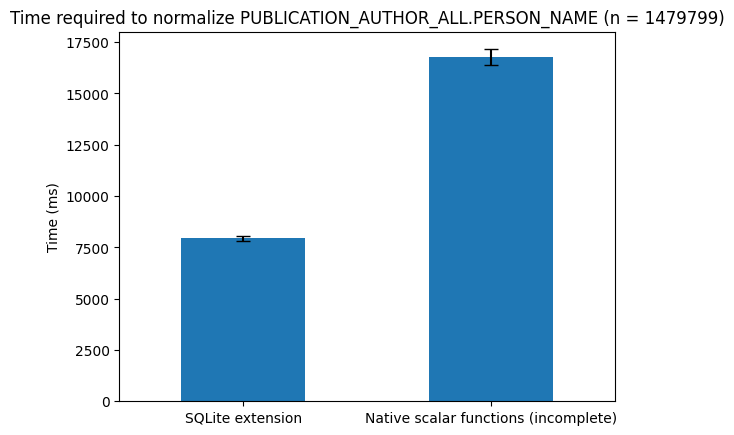
\includegraphics[width=\textwidth]{../img/sqlite_vs_native_scalar_functions.png}
    \centering
    \caption{The performance comparison of the SQLite extension and the composed scalar functions (mean over 10 runs).}
\end{figure}

After the normalization and aggregating the records using the normalized names,
we get \texttt{240001} distinct normalized names in the dataset.

% todo factcheck
The most frequent external author was \textit{B. Abbott} with $1339$ records, followed by $J. Smith$ with $1178$ records.
This raises concerns about the uniqueness of the normalized names - as with $1339$ coauthored publications, \textit{B. Abbott} would be the 99.9 percentile (or the top 7th author),
compared to the internal authors with known identifiers.

\textbf{Issues with the naïve approach}

While the naïve approach is simple and straightforward, it also has logical drawbacks.

In the current state, there is no support for the existing identifiers from the dataset.
By only inferring the identifier from the name, we willingly discard the existing information about the person.

This could be partially solved by concatenating the inferred identifier with the existing one. 
However, such approach would only fully work in the case of the external authors.
In the case of the internal authors with few records with missing identifiers (e.g. \hyperref[fig:jaroslav-peska]{Jaroslav Peška}),
this would still result in the creation of multiple nodes for the same person (e.g. \texttt{14124313-jaroslav-peska} and \texttt{null-jaroslav-peska}).

\subsubsection{(Distance-based) hierarchical clustering}

To solve the issues of the naïve approach, we can try to use the graph structure of the data to infer the missing identities.
One of the possible approaches is to use the \textit{hierarchical clustering} methods to group the nodes with similar attributes together.

\subsubsection{Embedding-based clustering}

Another approach to the problem of inferring the missing identities is to use the \textit{embedding-based clustering} methods.

The idea behind the embedding-based clustering is to project the nodes of the graph into a lower-dimensional space, where the nodes with similar attributes are close together.

The graph database Memgraph\footnote{\url{https://memgraph.com/}} offers a built-in implementation of the \textit{node2vec} algorithm\footnote{\url{https://snap.stanford.edu/node2vec/}}.
We can use this to project the nodes of the graph into a 2D space and then use the clustering algorithms to group the nodes with similar attributes (and same normalized names) together.


% \section{Inferring missing data}

% This section talks about the data inference for missing data. This is a problem mostly for the external authors (with little to no affiliation to CUNI) who can be often only identified by their name and academic titles. We try to come up with a better way of ``filling in the blanks'' - either by using some basic statistics or some data extracted from the social network itself.

% \subsection{Infering identities from the social network}

% Another example is the search for Dmytro Yu Balakin, which yields the following results:

% \begin{itemize}
%     \item Dmytro Yu Balakin
%     \item Dmytro Yu Batakin
%     \item Dmytro Yu. Balakin.
% \end{itemize}

% It is clear that most of those are likely the same person, but the data is not consistent. The first one is the correct one, but the other ones are missing the academic titles and the ``doc.'' prefix. The ``PhD.'' suffix is also inconsistent - sometimes it is ``PhD.'', sometimes ``Ph.D.''. The ``doc.'' prefix is also sometimes missing.

% ...
% ...

% While it might be tempting to solve this "online" by visually merging the entities in the application's visualization layer, this causes multiple issues. The obvious one are the performance implications 

% \section{Analyzing the social network}

% The first contact with the network, description of some basic properties, discovering the features of the data and trying to mine some non-obvious relations from the data.

% \dots